\documentclass[tikz,border=6pt]{standalone}
\usetikzlibrary{arrows.meta,calc,decorations.markings}
\usepackage{amsmath, amssymb, amsfonts}
\begin{document}
	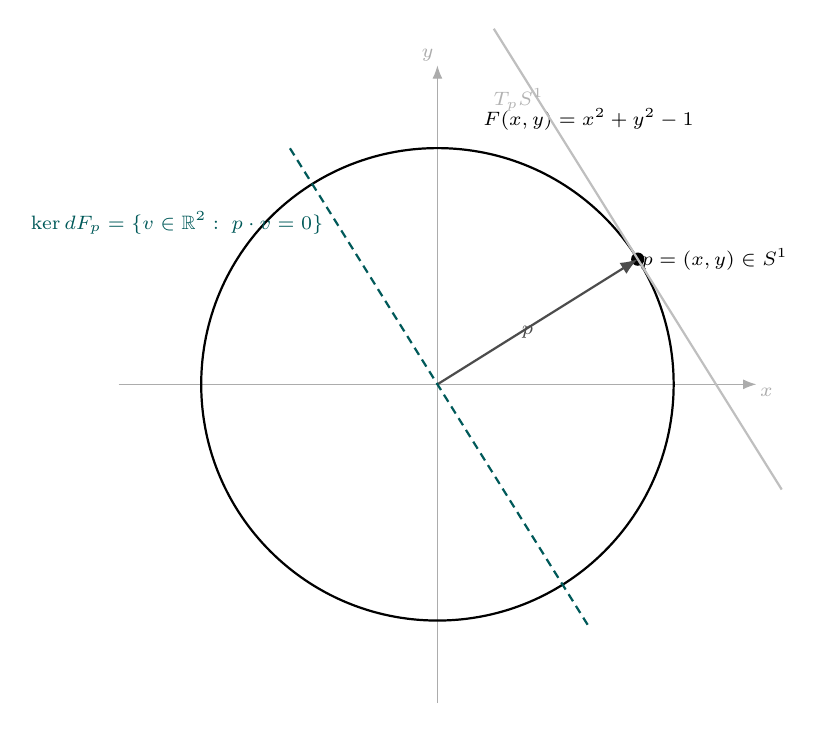
\begin{tikzpicture}[
		scale=3,
		axis/.style={thin,gray!65},
		vec/.style={-{Latex[length=2.2mm]},thick},
		tangent/.style={-{Latex[length=2mm]},very thick,orange!85!black},
		normal/.style={-{Latex[length=2mm]},very thick,blue!75!black},
		kerline/.style={densely dashed,thick,teal!70!black},
		circ/.style={thick,black},
		lab/.style={font=\scriptsize,inner sep=1.2pt}
		]
		% ===== Parameters =====
		\def\R{1}              % circle radius
		\def\a{32}             % angle (degrees) for point p on S^1
		% ===== Coordinates for p and Jp =====
		\pgfmathsetmacro{\px}{cos(\a)}
		\pgfmathsetmacro{\py}{sin(\a)}
		\pgfmathsetmacro{\jpx}{-sin(\a)} % Jp = (-y,x)
		\pgfmathsetmacro{\jpy}{cos(\a)}
		% convenient scalar for arrow lengths
		\pgfmathsetmacro{\Ltan}{0.38}
		\pgfmathsetmacro{\Lnor}{0.38}
		\pgfmathsetmacro{\Ltangrid}{1.15}
		% ===== Axes =====
		\draw[axis,-{Latex}] (-1.35,0) -- (1.35,0) node[below right,lab] {$x$};
		\draw[axis,-{Latex}] (0,-1.35) -- (0,1.35) node[above left,lab] {$y$};
		% ===== Unit circle: S^1 = {F=0} =====
		\draw[circ] (0,0) circle (\R);
		\node[lab] at (0.64,1.12) {$F(x,y)=x^2+y^2-1$};
		% ===== Point p and radius vector =====
		\fill (\px,\py) circle (0.8pt);
		\node[lab,anchor=west] at (\px,\py) {$p=(x,y)\in S^1$};
		\draw[vec,black!70] (0,0) -- (\px,\py) node[midway,below left,lab] {$p$};
		% ===== Tangent line at p (direction Jp) =====
		\draw[thick,gray!50]
		({\px - \Ltangrid*\jpx},{\py - \Ltangrid*\jpy})
		-- ({\px + \Ltangrid*\jpx},{\py + \Ltangrid*\jpy});
		\node[lab,anchor=south east,gray!60] at ({\px + 0.72*\jpx},{\py + 0.72*\jpy})
		{$T_pS^1$};
		% ===== Kernel line at the origin (same direction as Jp) =====
		\draw[kerline]
		({-1.2*\jpx},{-1.2*\jpy}) -- ({1.2*\jpx},{1.2*\jpy});
		\node[lab,anchor=north east,teal!70!black]
		at ({0.88*\jpx},{0.88*\jpy})
		{$\ker dF_p=\{v\in\mathbb{R}^2:\;p\cdot v=0\}$};
%		% ===== Tangent (Jp) and normal (2p) arrows at p =====
%		\draw[tangent] (\px,\py) -- ({\px + \Ltan*\jpx},{\py + \Ltan*\jpy})
%		node[pos=1,above right,lab] {$Jp=(-y,x)$};
%		\draw[normal] (\px,\py) -- ({\px + \Lnor*\px},{\py + \Lnor*\py})
%		node[pos=1,above,lab] {$\nabla F(p)=2p$};
%		% ===== Small curve gamma on S^1 through p with velocity parallel to Jp =====
%		\draw[very thick,red,
%		decoration={markings,mark=at position 0.62 with {\arrow{Latex}}},
%		postaction=decorate]
%		({cos(\a-24)},{sin(\a-24)}) arc[start angle=\a-24,end angle=\a+24,radius=\R];
%		\node[lab,red] at ({cos(\a-12)+0.04},{sin(\a-12)-0.06}) {$\gamma\subset S^1$};
%		\node[lab,red] at ({\px + 0.04*\jpx},{\py + 0.04*\jpy}) {$\gamma'(0)\parallel Jp$};
%		% ===== Algebraic labels =====
%		\node[lab,anchor=west,fill=white,draw=black!20]
%		at (-1.31,1.12)
%		{$dF_p=\begin{bmatrix}2x&2y\end{bmatrix},\quad
%			dF_p(u,v)=2xu+2yv$};
%		\node[lab,anchor=north east,fill=white,draw=black!20]
%		at (-1.05,-1.05)
%		{$T_pS^1=\ker dF_p\;\;=\;\{v:\;p\cdot v=0\}
%			\;=\;\operatorname{span}\{Jp\}$};
%		% ===== Tangency equation (optional label) =====
%		\node[lab,gray!60] at ({\px - 0.55*\jpx},{\py - 0.55*\jpy})
%		{$\;\;p\cdot q=1\;\;(\text{line through }p)$};
	\end{tikzpicture}
\end{document}
